\documentclass[12pt]{article}
\usepackage{graphicx}
\usepackage{amssymb,amsmath}
\usepackage{epstopdf}
\usepackage{natbib}
\usepackage{aas_macros}

\DeclareGraphicsRule{.tif}{png}{.png}{`convert #1 `dirname #1`/`basename #1 .tif`.png}
\textwidth = 6.5 in
\textheight = 9 in
\oddsidemargin = 0.0 in
\evensidemargin = 0.0 in
\topmargin = 0.0 in
\headheight = 0.0 in
\headsep = 0.0 in
\parskip = 0.2in
\parindent = 0.0in

\def\Response{R_{yn}}
\def\ResponseMatrix{R}


\title{The Music of the Sphere: Inferring the Evolution of the Universe on the Largest Scale from Cosmic Microwave Background Observations and Deep Survey Data.}
\author{Roger D. Blandford, Philip J. Marshall, Laurence Perreault-Levasseur}

\begin{document}

\maketitle

\section{Overview}
Observations of temperature fluctuations in the CMB measure the 2D potential $\Phi$ (considered as a linear perturbation to the Robertson-Walker metric tensor under the Newtonian gauge) on the sphere of last scattering (where the scale factor $a\sim0.0009$ and the time is $t\sim380$~kyr). The measurement is quite direct on large angular scale ($\ell\lesssim30$) in the ``Sachs-Wolfe'' regime; it is indirect on small angular scales where velocity and density perturbations are more important, which are linearly related to the potential perturbation. It is also possible, at least in principle, to learn about the first and second radial derivatives of this potential through studying the polarization. This 2D potential is derived from a 3D potential which fills the sphere and extends beyond our horizon. This potential is derived from one specific realization of an initial Fourier spectrum of inferred type and statistical properties.  This paper reports on an investigation of what can be learned, at least in principle, about the 3D potential at the time of recombination from the 2D information. Furthermore, any set of Fourier components can be evolved assuming the now standard ``Flat $\Lambda$ CDM'' cosmology and connected to the potential information derivable from large surveys conducted out to modest redshift. What is being discussed here is an exercise in basic cartography and not in measuring the physical behavior of the universe at either early or late times. As with many such exercises the goal is to understand the approximate arrangement of structure within the observable universe on the largest linear scales. We shall be more concerned with the topological organization of this structure than with precise measurement. However, success in this endeavor ought to improve the investigation of physics questions through contributing constraining priors to Bayesian inference studies.

In Sec. 2, we discuss the basic assumptions that we will make in our idealized versions of the problem. This is followed in Sec. 3 by a description o fate Fourier representation of the 3D potential and its relationship to the spherical harmonic decomposition on the last scattering sphere. The nesting of equipotential contours on the last scattering photosphere is analyzed in Sec. 4 and this is generalized to surfaces in 3D in the following section.  The relationship between the 2D and 3D equipotentials is discussed in Sec.6. In Sec. 7., we outline a Bayesian approach to calculating the likeliest form of the 3D potential, paying special attention to the criteria which dictate the effective resolution of the reconstruction and how this may be improved by adding interior data. Our conclusions are collected in Sec. 8. A future publication will apply this approach to actual data.

\section{Basic Assumptions}
We  work with an idealized problem which we specify as follows:
\begin{itemize}
\item Represent the big bang as a sphere of comoving radius $\sim14.23$~Gpc (adopting a Hubble constant of 68 km s$^{-1}$ Mpc$^{-1}$) and flat $\Lambda$CDM .  The last scattering surface -- the \emph{cosmic photosphere} --  is a sphere with radius $\sim0.29$~Gpc smaller. Recombination occurs over a short but finite interval of time just prior to last scattering. The radius of the cosmic photosphere, 13.94~Gpc, is our unit of length.
\item Ignore the expansion of the universe and just consider the potential as a set of linear normal modes at the time of last scattering. These can be evolved backward and forward in time with confidence. In practice, the potential changes little after recombination although shorter-wavelength modes eventually become nonlinear. (This, too, can be accommodated in principle.)
\item Consider only scalar modes, setting the tensor contribution to zero. If, one day, a significant tensor component is confidently measured, minor modifications to what follows can be included.
\item Hypothesize that the amplitude of each of these modes is drawn from a Gaussian distribution with zero mean, random phase and initial variance roughly proportional to $k^{-3}$ as is consistent with the observations.
\item Ignore modes with wavelength longer than the side of the box, {L}. Their contributions can be approximately incorporated into the lowest Fourier components in a given box as long as we only care about observations within our horizon. This procedure will improve as we enlarge the box. However if the box is too large the spacing of modes in k-space $\Delta k=2\pi/L$ will be too fine and the amplitudes of neighboring modes will be poorly distinguished. A choice $L\sim4$ turns out to be a good compromise. Truncate the spectrum with a sphere of radius $n_{\rm max}\Delta k$; shorter wavelength modes contribute to the error and a Gaussian window function may be preferable.
\end{itemize}

\section{Fourier Modes}
We represent the potential $\Phi$ within the box in polar coordinates as a Fourier series with wave vectors ${\bf k}=\Delta k\{n_1,n_2,n_3\}$, with $n_1,n_2,n_3$ integers and $\Delta k=2\pi/L$. As $\Phi$ is real, we only need to assign one real number to each mode. We approximate Eq.~(1) by a finite sum restricted to $(n_1^2+n_2^2+n_3^2)^{1/2}\le n_{\rm max}$ and we label the coefficients $f_{\bf k}$ by the index $n$ running from $1$ to $N\sim4\pi n_{\rm max}^3/3$. ($N=6,32,122, 256,514,924,1418,2108,3070,4168$ for $n_{\rm max}=1$ through $10$.) It is simplest to restrict ${\bf k}$ to a hemisphere and to write:
\begin{equation}
\Phi[{\bf x}(x,\theta,\phi)]=\sum_{n=1}^{N/2}[f_n\cos({\bf k}_n\cdot{\bf x})+f_{N+1-n}\sin({\bf k}_n\cdot{\bf x})]
\end{equation}
\begin{figure}[h!]
\centering
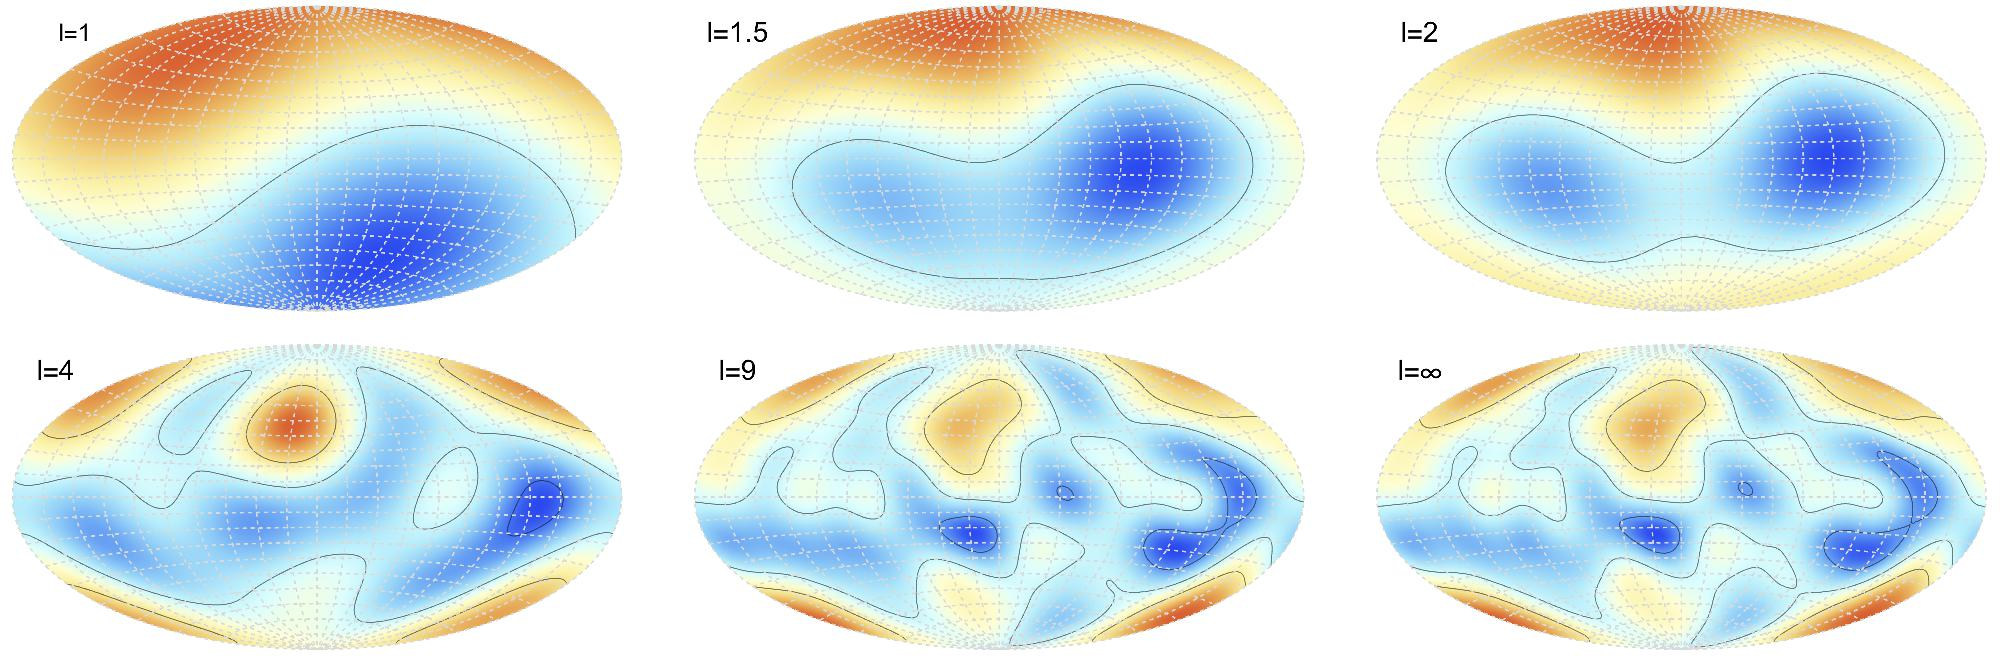
\includegraphics[width=6in]{fig1.jpg}
\caption{Aitoff projections of the potential on the cosmic photosphere $\Phi(\theta,\phi;\ell)$ at $x=1$ for different angular resolutions, parametrized by $\ell$. The contour levels are $0\pm1$. A fixed set of random Fourier components truncated with $n_{max}=3$ is used.}
\end{figure}

<<<<<<< HEAD
Our first goal is to relate the interior potential to the photospheric measurement.\footnote{This is sometimes called \emph{holography}, though it is not the original meaning of the word.} The approach that we will follow is constructive. The potential, $\Phi({\bf x})$ can be expanded exactly as an infinite sum of Legendre polynomials which we truncate at a finite value of $\ell$ to furnish an approximation:
=======
Our main goal is to relate surface information on the photosphere to the underlying $f_n$.\footnote{This is sometimes called \emph{holography}, though it is not the original meaning of the word.} The approach that we will follow is constructive. $\Phi$ can be expanded exactly as an infinite sum of Legendre polynomials which we truncate at a finite value of $\ell$, starting with $\ell=1$.
>>>>>>> 57b82e01c37c3b842dec4bc1bdd7961c5aa226d1
\begin{equation}
\Phi({\bf x;\ell})=\sum_{\ell'=0} ^\ell(2\ell'+1)\sum_{n=1}^Nj_{\ell'}(k_nx)P_{\ell'}({\hat{\bf k}}_n\cdot{\hat{\bf x}}){\cal S}(n,\ell')f_n,
\end{equation}
where ${\bf k}_n={\bf k}_{N+1-n}$ and ${\cal S}(n,\ell)=[\cos(\ell\pi/2),\sin\ell\pi/2)]$, for $[1\le n\le N/2,N/2<n\le N]$. As $\ell$ is increased the effective resolution of $\Phi$, in radius and angle, improves. It is convenient to treat $\ell$ as a continuous variable by the device of summing up to $\lfloor\ell\rfloor$  and then adding the next term in the sum multiplied by $(\ell-\lfloor\ell\rfloor)$. To describe the potential generated by modes with a given value of $n_{\rm max}$, we need spherical harmonics up to $\ell\sim3n_{\rm max}$ and {\it vice versa} (Fig.~1). An immediate implication is that an accurate $\Phi$ map on the sphere, degraded to resolution $\ell$ provides $L=(\ell-1)(\ell+3)$ real numbers which can be used to solve for $N$ real Fourier coefficients suggesting that there is enough information in a $\ell=9$ map to solve for $\sim100$ Fourier components up to $n_{\rm max}\sim3$ independent of the priors on their actual values. When we include the priors, we can proceed to finer scale. Also, when we reduce the radius of the sphere, the value of $n_{\rm max}$  probed by a given $\ell$ scales $\propto x^{-1}$ (Fig. 2).

\begin{figure}[h!]
\centering
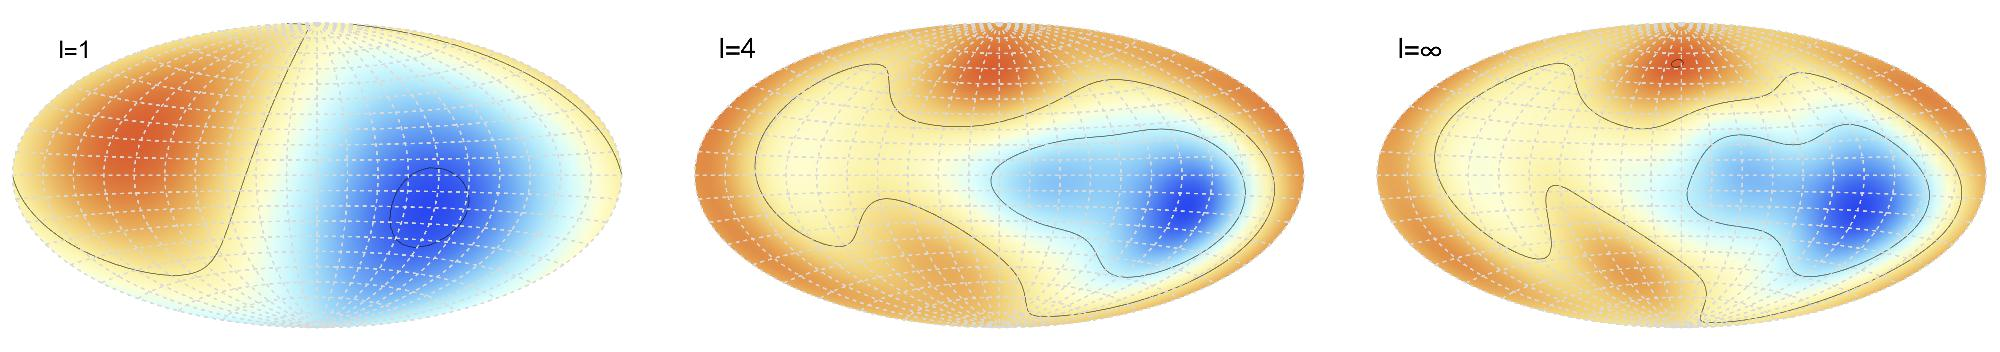
\includegraphics[width=6in]{fig2.jpg}
\caption{Aitoff projections of the potential on a sphere with $x=0.5$ with the same Fourier series as in Fig.~1. The expansion up to $\ell=4$ is a very good approximation to the full potential.}
\end{figure}

\section{Nesting of Equipotential Lines on the Sphere}
Analyze the potential on the cosmic photosphere ($x=1$) in a way that will generalize to the 3D potential in the sphere. The $\ell=0$ term is just a constant and, although necessary for the expansion we have just described, can be ignored here.  The $\ell=1$ surface potential $\Phi(\ell,\theta,\phi)$ develops a single simple minimum (henceforth designated as $L_0$) and single simple maximum (henceforth designated by $H_0$). These are the global  minimum and maximum; additional higher and lower minima and maxima will be designated $L_i$ and $H_i$ respectively in the order in which they appear.
\subsection{Classification of saddles}
Now gradually increase $\ell$. One contour develops a simple \emph{saddle}\footnote{We are interested in \emph{non-degenerate} critical points and exclude \emph{degenerate} extrema like \emph{monkey saddles} which are structurally unstable and unfold into simple extrema under a small perturbation.} and an extremum simultaneously, becoming a \emph{separatrix}. This contour divides the sphere into an \emph{inside} containing $L_0$ and \emph{outside} containing $H_0$. When the new extremum is a $L$ lying outside the contour, the separatrix/saddle combination has the shape of an infinity symbol and called a \emph{lemniscate}, denoted by $X$; when it is a $H$ lying inside the contour, the separatrix/saddle combination has the shape of a pinched annulus and is called a \emph{lima\c con}, denoted by $K$ (Fig.~3). As $\ell$ is further increased, the two stationary points separate and the smaller loop grows in size.\footnote{Note that had we associated the interior with $H_0$, a given contour would have had the opposite identification.} Further increasing $\ell$ will lead to the \emph{creation} of new separatrices. These may be located between two existing separatrices or out of a contour encircling a $L$ or a $H$.  Occasionally, the inverse process - \emph{annihilation} will occur. If we designate the total  number of maxima, minima, saddles, lemniscates and lima\c cons by $N_H,N_L,N_S,N_X,N_K$, respectively, then clearly $N_S=N_X+N_K=N_H+N_L-2$.

\begin{figure}[h!]
\centering
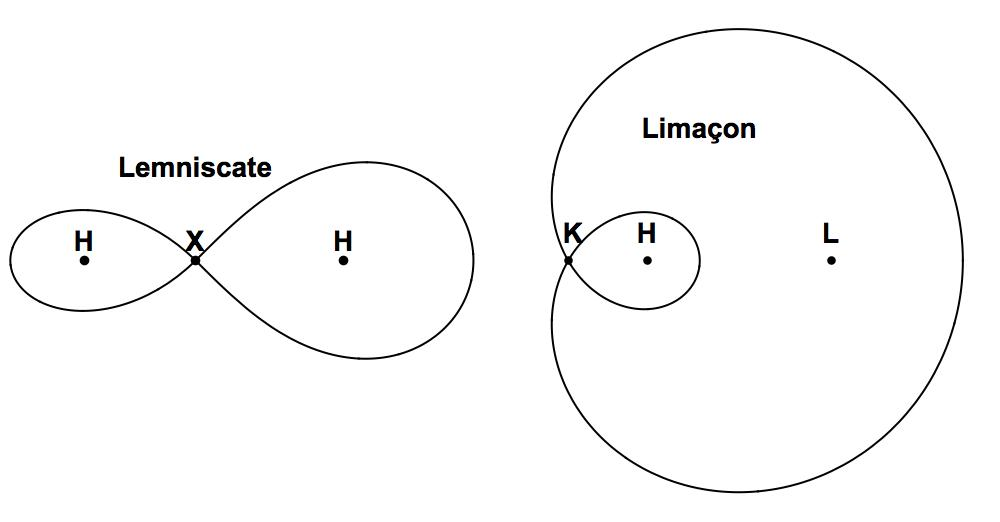
\includegraphics[width=4in]{fig3.jpg}
\caption{Two elementary types of saddle as characterized by the shape of the separatrix -- the equipotential passing through the saddle. The lemniscate, or $X$-saddle, is accompanied by two maxima $H$ , as here, or two minima, $L$. The \emph X may be created or annihilated with an extremum by growing or shrinking either of the closed loops that passes through it. The lima\c con, or $K$-saddle, is accompanied by a $H$ as here (or a $L$) and a $L$ as here (or a $H$). It can be create or annihilated only with one of the two accompanying extrema, in this case the $H$, so long as the contour does not expand and pass around the back of the sphere.}
\end{figure}

\subsection{Tree representation}
The nesting of all of the separatrices suffices to describe the nesting of all of the equipotentials. It is convenient to represent this nesting using a type of \emph{directed graph} or \emph{tree} representation. A simple example of a nesting is shown in Fig.~4a and the associated tree is presented in Fig.~4b.  The tree comprises \emph{nodes} or \emph{vertices}, each with three \emph{branches} or \emph{edges}, each corresponding to a separatrix and \emph{leaves} at the end of a branch corresponding to local extrema. There is only one path connecting any two leaves and no circuits, consistent with the usual definition of a tree. However, our tree has some novel features including growth.  We start with $\ell=1$ and a single branch from the $L$ (the \emph{root}) to the $H$ (the \emph{apex}). We let the vertical height of the branch be the potential difference between the two extrema. as we increase $\ell$, new node-leaf (saddle-extremum) pairs appear and we locate them with ordinates corresponding to their respective potentials. The $X$- and $K$-saddles are easily distinguished. The pre-existing nodes and leaves will also move and occasionally they may disappear; they may also pass through each other on a branch when their heights coincide. The horizontal separation of the nodes and leaves is adjusted to ensure that there are no crossovers; it has no quantitative significance. This description of the equipotentials is essentially topological and pays no attention to the actual location of the contours.

\begin{figure}[h!]
\centering
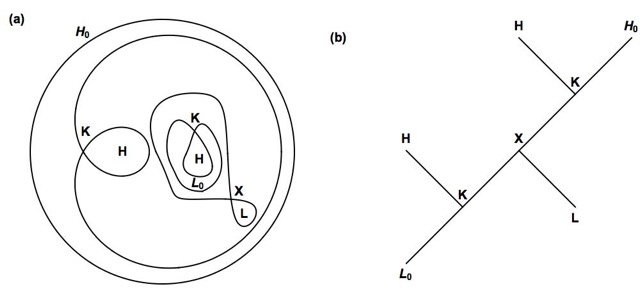
\includegraphics[width=6in]{fig4.jpg}
\caption{(a) Nesting of separatrices  exhibited within a circle created by puncturing the sphere at the global maximum and stretching the surface to lie on a plane so that the circumference is identified with a single point. b) Same separatrices displayed on a sphere. (c) Tree representation of this nesting. The designation of the saddles $X$, $K$ and the extrema, $H$, $L$, is redundant and can be dropped. The numbers designate the order in which the extrema appear as $\ell$ is increased.}
\end{figure}

\subsection{Stationary points}
Finding all the stationary points can be difficult.  The simplest approach is to set $\nabla_2\Phi=\Phi_{ij}=\{\partial\Phi/\partial{\hat\theta},\partial\Phi/\partial{\hat\phi}\}$ to zero, using the identity $P_\ell'(\mu)=\ell[P_{\ell-1}(\mu)-\mu P_\ell(\mu)]/(1-\mu^2)$ and differentiating the sums in Eq.~2. This defines two families of curves and the stationary points are located where they intersect. New stationary points appear when these curves first touch.\footnote{In the language of catastrophe theory , this is a fold catastrophe.} An alternative method, which works well, is to find local minima of $|\nabla_2\Phi|^2$.

\subsection{Curvature maps}
There is another way to discuss the critical points and this is to evaluate the Hessian matrix
\begin{equation}
H_{ij}=\Phi_{,{\hat i}{\hat j}}
\end{equation}
where the derivatives are with respect to $\hat\theta$, $\hat\phi$. It is straightforward to compute the two real eigenvalues which represent the principle curvatures. We can then designate $L$-zones, where they are both negative, $H$-zones, where they are both positive and $S$-zones  where they have opposite signs. (We can further subdivide these zones dependent upon which eigenvalue has the larger absolute value but will not do this here.)  As can be seen in Fig.~5, $H$ and $L $ zones have common boundaries with $S$, where one eigenvalue changes sign and touch at points where both eigenvalues simultaneously pass through zero.  New saddle-extremum pairs are created at saddle boundaries and then quickly separate into their respective zones. This provides an alternate means to locate new separatrices. Individual curvature zones can contain multiple or no stationary points.

\begin{figure}[h!]
\centering
%\includegraphics[width=6in]{fig5.jpg}
\caption{Division of sphere into curvature zones. The $L$-zone is denoted in blue, the $H$-zone in red and the $S$-zone in purple. Also shown are the lines where the two components of $\nabla\Phi$ vanish. Their intersections correspond to stationary points.}
\end{figure}

\subsection{Curve of growth}
The number of extrema, measured by the number of saddles $N_S$ increases with $\ell$. The manner in which it does this is dictated by the slope of the power spectrum of potential fluctuations $P_{\bf k}$ though not it's amplitude. We have focused on the inverse cube case because this is close to the inferred initial spectrum and remains valid around recombination up to $\ell\sim30$. (It is also the spectrum for the temperature perturbations because the gravitational redshift is the dominant effect in the \emph{Sachs-Wolfe} regime.) General scaling arguments suggest that as long as $P(k)\propto k^{n-4}$ for fixed $n$ then the expectation in the number of saddles counted when all $N_S(\ell)$ is given asymptotically by $K(n)\ell^2$ as $\ell\rightarrow\infty$ where $K$ can be estimated using a large number of  trials. The variance in the actual value of $K$ for finite $\ell$ can also be computed. We can also apply this approach directly to the temperature fluctuations assuming the inferred fluctuation spectrum inferred by more conventional methods. This will be demonstrated in a subsequent publication but is no more than a consistency check.

\subsection{Gaussianity}
We have considered several ways to classify the extrema and the results can be used to check on the Gaussianity of the distribution of Fourier components. For example, if the distributions of the Fourier coefficients were systematically skewed, then we would expect differences in the numbers of $L$ and $H$ and the areas of the corresponding zones. More subtle tests are possible using the branching of the trees. These will be considered elsewhere and compared with the observations.

\section{Nesting of Equipotential Surfaces in the Sphere}

\section{Relating Surface and Interior Equipotentials}
Now let us outline how to extract information about the interior potential from the surface potential. We suppose that we are in the Sachs-Wolfe region of the spectrum where the surface potential $\Phi(1,\theta,\phi)=3\delta_T$, where $\delta_T$ is the relative CMB fluctuation. We set aside for the moment the velocity and density contributions to the observed fluctuation and the additional information (roughly twice as much) that can be garnered from adding  polarization maps. We align the 3 axis (Eq.~(1)) with $\theta=0$ and the 1 axis with $\phi=0$.

Our first task is to describe the inferred potential on the sky. We suppose this is approximated by a finite sum over spherical harmonics:
\begin{equation}
\Phi(1,\theta,\phi;\ell_{\rm max})=\sum_{y=1}^{(\ell_{\rm max}+1)^2}a_yY_y(\theta,\phi),
\end{equation}
where $Y_y=\{Y_{0,0},Y_{1,0},2^{1/2}\Re[Y_{1,1}],2^{1/2}\Im[Y_{1,1}],Y_{2,0},\dots,2^{1/2}\Im[Y_{\ell_{\rm max},\ell_{\rm max}}]\}$. Note that there are $2\ell+1$ independent, real, basis function in each $\ell$-shell. Note also that $\int d\Omega Y_yY_{y'}=\delta_{yy'}$.

Next, we describe the potential using Eq.~(2) and the identity
\begin{equation}
P_{\ell}[\hat{\bf k}(\theta',\phi')\cdot\hat{\bf x}(\theta,\phi)]=\frac{4\pi}{2\ell+1}\sum_{y=\ell^2+1}^{(\ell+1)^2}Y_y(\theta',\phi')Y_y(\theta,\phi)
\end{equation}
The spherical harmonic coefficients are then given by the linear relation
\begin{equation}
a_y=\Response f_n,
\end{equation}
where we adopt the summation convention and
\begin{equation}
\Response =4\pi i^\ell Y_y^\ast(\theta',\phi')j_\ell(k),
\end{equation}
with $\cos\theta'=n_3/n,\tan\phi'=n_2/n_1$. The elements of the transformation matrix $\Response$ have been tabulated up to $n_{\rm max}=6$, $l=10$ which should be sufficient for our purpose.

We estimate the importance of spherical harmonics with order $\ell$ to the signal at a given given range of $k$ by evaluating the sum:
\begin{equation}
P(\ell;n_{\rm max})=\sum_{n=N(n_{\rm max}-1)+1}^{N(n_{\rm max})}\sum_{y=\ell^2-3}^{(\ell-1)(\ell+2)}|\Response|^2
\end{equation}
\begin{figure}[h!]
\centering
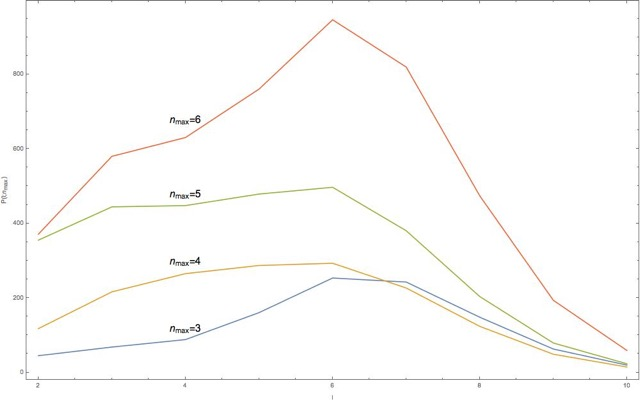
\includegraphics[width=6in]{fig6.jpg}
\caption{Importance of spherical harmonics of order $\ell$ for shells in k-space with inner radius $n_{\rm max}-1$ and outer radius $n_{max}$.}
\end{figure}

\section{Inferring the 3D Potential}

Our task is to take a given vector of measured spherical harmonic
coefficients $\mathbf{a}$, with covariance matrix $C$,  and
infer a vector of the Fourier coefficients of our model potential,
$\mathbf{f}$,  under the prior assumption that the  components $f_n$
are independent and drawn from a Gaussian distribution with variance
$\sigma_n^2 = (n_1^2+n_2^2+n_3^2)^{-3/2} / \alpha$. We seek the
posterior PDF ${\cal P} = \Pr(\mathbf{f}|\mathbf{a},\alpha)$, where
\begin{equation}
% -\ln{\cal P} = \frac{(a_y^2-\Response f_n)^2}{2\sigma_y^2}+\frac{f_n^2}{2\sigma_n^2} + \text{const.}
-\ln{\cal P} = (\mathbf{a}-\ResponseMatrix\mathbf{f})^{\rm T} C^{-1} (\mathbf{a}-\ResponseMatrix\mathbf{f})
             + \mathbf{f}^{\rm T} S^{-1} \mathbf{f} + \text{const.}
\end{equation}
and the matrix $S$ is diagonal, with
elements~$S_{nn} = \sigma_n^2$.
Differentiating this expression leads to a set of linear equations
% \begin{equation}
% \left(\frac{\Response m_{yn'}}{\sigma_y^2}+\frac{\delta_{nn'}}{\sigma_n^2}\right)f_{n'}=\frac{a_y\Response}{\sigma_y^2},
% \end{equation}
which can be solved for the maximum posterior 3D potential
Fourier coefficients $\mathbf{f}_{\rm MP}$, given a choice of power spectrum
normalisation~$\alpha$. We follow \citep{SuyuEtal2006} and infer the
most probable normalisation~$\alpha_{\rm MP}$ using the Bayesian Evidence,
which leads to the approximate condition
\begin{equation}
    (\mathbf{a}-\ResponseMatrix\mathbf{f}_{\rm MP})^{\rm T} C^{-1} (\mathbf{a}-\ResponseMatrix\mathbf{f}_{\rm MP})
                 + \mathbf{f}_{\rm MP}^{\rm T} S^{-1}(\alpha) \mathbf{f}_{\rm MP} \approx N/2
\end{equation}
where $N$ is the number of spherical harmonic coefficients used. An
iterative scheme was used to optimize $\alpha$ in this way.

We note that the covariance matrix of the measured spherical harmonic
coefficients should not include any cosmic variance terms, because we
are interested in inferring the 3D potential in our one observable
universe. To estimate this object, we took 100 posterior sample
``Commander-Ruler'' temperature maps, decomposed each of them into
spherical harmonics,\footnote{We use the {\sc healpy} code provided at
\texttt{https://healpy.readthedocs.org}.} and then calculated the
sample variance and sample covariance of the coefficients.


\section{Discussion}


\bibliographystyle{apj}
\bibliography{references}


\end{document}


\begin{eqnarray}
\Phi(x,\theta,\phi)&=&8\pi\sum_{\ell=0,2,\dots}^\infty(-1)^{\ell/2}\sum_{\bf k}^{\cal H}\Re[{\tilde\Phi}_{\bf k}]j_\ell(kx)\sum_{m=-\ell}^\ell Y_{\ell m}^\ast(\theta',0)Y_{\ell m}(\theta,0)\cos[m(\phi-\phi')]\cr
&+&8\pi\sum_{\ell=1,3,\dots}^\infty(-1)^{(\ell+1)/2}\sum_{\bf k}^{\cal H}\Im[{\tilde\Phi}_{\bf k}]j_\ell(kx)\sum_{m=-\ell}^\ell Y_{\ell m}^\ast(\theta',0)Y_{\ell m}(\theta,0)\cos[m(\phi-\phi')].
\end{eqnarray}

where ${\bf k}=\pi[n_1,n_2,n_3]=k[\sin\theta'\cos\phi',\sin\theta'\sin\phi',\cos\theta']$, with $n_1,n_2,n_3$ integers and ${\bf x}=x[\sin\theta\cos\phi,\sin\theta\sin\phi,\cos\theta]$.  As $\Phi$ is real, we know that ${\tilde\Phi}_{\bf k}(-{\bf k})={\tilde\Phi}^\ast_{\bf k}({\bf k})$ and so we only need define the Fourier components over a hemisphere $\cal H$ in ${\bf k}$ space. We choose ${\cal H}=\{n_1>0\}\cup\{n_1=0,n_2>0\}\cup\{n_1=n_2=0,n_3>0\}$.


\begin{eqnarray}
\Phi(\bf x)&=&2\sum_{\bf k}^{\cal H}{\tilde\Phi}_{\bf k}\sum_{\ell=0}^\infty (2\ell+1)i^\ell P_\ell({\hat{\bf k}}\cdot{\hat{\bf x}})j_\ell(kx)\cr
&=&8\pi\sum_{\bf k}^{\cal H}{\tilde\Phi}_{\bf k}\sum_{\ell=0}^\infty i^\ell j_\ell(kx)\sum_{m=-\ell}^\ell Y_{\ell m}^\ast(\theta',\phi')Y_{\ell m}(\theta,\phi)
\end{eqnarray}

 Let us start with the monopolar ($\ell=m=0$) term in Eq.~(3). For the moment, we just explore the partial potential associated with this single term, $\Phi^{00}({\bf x})=\sum{\tilde\Phi}^{00}_{\bf k}e^{i{\bf k}\cdot{\bf x}}$. We can expand this in terms of the original Fourier coefficients as ${\tilde\Phi}^{00}_{\bf k}=M^{00}_{\bf kk'}{\tilde\Phi}_{\bf k'}$, where $\bf k$, $\bf k'$ are shorthand for all the indices that specify individual spatial modes (summed when repeated) and we allow the matrix $M^{00}$ to pick out the real part of $\tilde\Phi_{\bf k}$. In this case,
\begin{equation}
M^{00}_{\bf kk'}=\frac14\int d{\bf x}{\rm sinc}kx\cos{\bf k'}\cdot{\bf x},
\end{equation}
which is best evaluated numerically. We proceed in this manner to evaluate all the necessary matrix elements $M^{\ell m}_{\bf kk'}$. (Of course there is an infinity of function spaces we could have chosen.)

The strategy, then, is to start with a set of Fourier coefficients, $\tilde\Phi_{\bf k}$ which defines $\Phi({\bf x})$ within the box to sufficient resolution. We then use Eq.~(3) to define partial potentials associated with each spherical harmonic and sum them over $m$ to get a unique partial potential associated with each value of $\ell$. We then sum over all $\ell\le\ell_{\rm max}$ to give a low resolution version of the full potential which we designate as $\Phi(\ell_{\rm max},{\bf x})$. The benefit of this seemingly cumbersome procedure is that we do not have to include large values of $\bf k'$ for it to resemble an appropriately  smoothed version of the full potential and it accurately recovers the 2D potential as defined on the cosmic photosphere of radius $x_\gamma$. Conversely, as we increase $\ell_{\rm max}$, we converge quickly to the true potential at lower spatial resolution (Fig. ~1). An important point for what follows is that we can treat $\ell_{\rm max}$ not as an integer but as a continuous variable simply by adding a constant fraction in $\{0,1\}$  of all the $m$ components associated with $\ell=\ell_{\rm max}$.

We now repeat this exercise for the equipotential surfaces within the sphere. The structurally stable stationary points in 3D are again highs (the Hessian has three negative eigenvalues), lows (three positive eigenvalues) and saddles (both signs). The separatrices are now surfaces passing through the saddles. Close to the saddles, they take the form of two cones with a common vertex on the saddle.

What we must actually do first is to consider the equipotentials defined within the fundamental box with periodic boundary conditions so that opposite faces are identified. It is easy to see that the minimum number of stationary points in three dimensions is eight (six saddles a high and  a low). However, if we start with a sphere of sufficiently small radius, $x<1$ and $\ell=1$, there will be no stationary points within the sphere. We can then increase $x$ to unity bringing in additional stationary points. Next we increase $\ell$ as we did on the sphere. Provided that we consider the entire cube, each saddle is created with an accompanying $H$ or $L$.
